\section{Results}\label{sec:results}
Results are reported by hypothesis. Unless stated otherwise, values are means over ten paired seeds, and $p_H$ is the Holm-adjusted Wilcoxon $p$-value. Table~\ref{tab:hypotheses} at the end of the section summarizes the decisions.

\subsection{H1: Reproduction of DIS-FDM}
The reproduction confirmed DIS-FDM's effect on control overhead. With five attackers flooding every 3~s, DIO messages rose from 1245 without attack to 10\,451, and DIS-FDM cut them to 2348, below RPL-MRC's 3597. The published values show the same directions and the same ranking (590, 4080, 673, and 692) \cite{prajisha2025}. Four of the eight checked effect directions were reproduced, all four concerning overhead and defense ranking.

The other four concerned delivery, delay, and power. The base paper reported that DIS flooding lowered PDR from 97\% to 70.9\%; in our network, PDR stayed above 99.9\% with or without the flood, and delay and power did not change. The reason is the MAC layer. Our nodes run CSMA with the radio always on, so they absorb the extra DIOs without congestion, and power is dominated by listening (about 60~mW in every condition). The base paper's absolute values point to a duty-cycled radio, which we could not confirm because its MAC configuration is not reported. The reproduced mechanism (DIOs triggered by DIS and suppressed by DIS-FDM) is the one AEF-RPL builds on, so the extension rests on a validated base.

The sensitivity study also exposed a property of DIS-FDM that its published evaluation does not report. With its 10~s window, DIS-FDM detected no attackers flooding every 15 or 30~s, because a slow flood never produces consecutive window exceedances. A 30~s window recovered mean TPRs of 98\% and 88\%, at the cost of detection delays near 159 and 192~s. H1 is partly supported.

\subsection{H2: Damage of the Combined Attack}
Fig.~\ref{fig:damage} shows that the two mechanisms damage different parts of the network. Without a defense, DIS flooding alone raised DIO traffic but left downward delivery almost intact, while DAO manipulation alone cut downward delivery and left DIO traffic near its normal level. The combined attack imposed both costs at once. Compared with DIS flooding alone, it lowered downward PDR and ARI in all six conditions ($p_H\le.006$); at 14 attackers in static networks, ARI fell from 0.999 to 0.460. Compared with DAO manipulation alone, it raised DIO traffic in five of six conditions ($p_H\le.047$).

The combined attack was not worse than DAO manipulation in delivery (0 of 6 conditions), and it did not produce more DIOs than DIS flooding. The damage was therefore additive rather than amplified: each mechanism contributed its own cost, and neither made the other stronger. This matters for defense design. A defense must address both planes, because addressing one leaves the other cost fully in place. H2 is partly supported: the combined attack is worse than each single attack on the dimension that attack does not touch.

\begin{figure*}[t]
\centering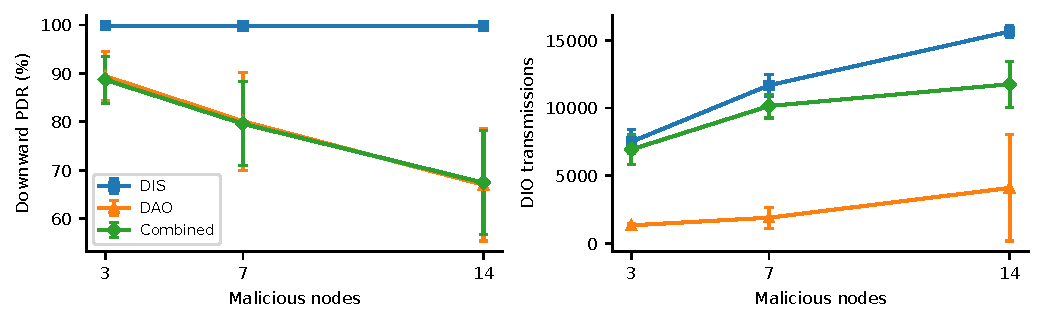
\includegraphics[width=.92\textwidth]{full_paper/generated/attack_damage.pdf}
\caption{Impact of DIS, DAO, and combined attacks on unprotected static networks across attacker counts (means and 95\% confidence intervals, ten seeds). DIS flooding raises DIO traffic; DAO manipulation lowers downward delivery; the combined attack does both.}\label{fig:damage}
\end{figure*}

\subsection{H3: DAO Evidence and Repair Against the Combined Attack}
Table~\ref{tab:mainresults} reports the seven-attacker comparison and Table~\ref{tab:primary} the tests across all six conditions. AEF-RPL raised downward PDR and ARI over DIS-FDM in every condition, all at the smallest attainable $p_H=.012$; ARI improved in every seed of every condition (rank-biserial correlation 1.0). With seven attackers in static networks, downward PDR rose from 77.2\% to 98.3\% and ARI from 0.71 to 0.92; with 14 attackers, ARI rose from 0.44 to 0.76. AEF-RPL's downward PDR was also significantly higher than that of Li-MSD, Secure-RPL, and RPL-MRC in all six conditions ($p_H=.012$). Service recovered more often as well: with seven attackers, downward service returned to 90\% of its pre-attack level in 7 of 10 static runs and 6 of 10 mobile runs with AEF-RPL, against 3 and 1 with DIS-FDM.

\begin{table}[t]
\caption{Combined attack with seven attackers (seeds 1--10). Mean $\pm$ 95\% confidence half-width, in percent.}\label{tab:mainresults}
\centering\footnotesize\setlength{\tabcolsep}{4pt}\begin{tabular}{@{}lrrrr@{}}
\toprule
Mobile (\%) & Method & Down PDR (\%) & TPR (\%) & FPR (\%) \\
\midrule
0 & RPL & 79.6$\pm$8.7 & -- & -- \\
0 & Secure-RPL & 77.4$\pm$12.1 & 97.1$\pm$6.5 & 0.0$\pm$0.0 \\
0 & DIS-FDM & 77.2$\pm$11.1 & 97.1$\pm$6.5 & 8.6$\pm$7.7 \\
0 & Li-MSD & 82.3$\pm$6.6 & 94.3$\pm$7.1 & 0.0$\pm$0.0 \\
0 & AEF fixed & 97.4$\pm$3.3 & 97.1$\pm$6.5 & 7.7$\pm$9.6 \\
0 & AEF learning & 98.3$\pm$1.6 & 97.1$\pm$6.5 & 16.8$\pm$15.4 \\
30 & RPL & 82.6$\pm$12.0 & -- & -- \\
30 & Secure-RPL & 80.8$\pm$11.1 & 100.0$\pm$0.0 & 0.0$\pm$0.0 \\
30 & DIS-FDM & 80.8$\pm$11.3 & 100.0$\pm$0.0 & 69.5$\pm$17.3 \\
30 & Li-MSD & 85.7$\pm$11.2 & 65.7$\pm$15.4 & 2.7$\pm$2.3 \\
30 & AEF fixed & 98.1$\pm$1.3 & 100.0$\pm$0.0 & 54.5$\pm$11.9 \\
30 & AEF learning & 96.4$\pm$3.8 & 100.0$\pm$0.0 & 55.0$\pm$12.6 \\
\bottomrule
\end{tabular}

\end{table}

\begin{table*}[t]
\caption{AEF-RPL against DIS-FDM under the combined attack in all six conditions ($k$ attackers; S static, M 30\% mobile), and learning against the fixed rule for detection latency. Means over ten paired seeds; $p_H$ is the Holm-adjusted two-sided Wilcoxon $p$-value. Recovered: runs (of ten) in which downward service returned to 90\% of its pre-attack level.}\label{tab:primary}
\centering\footnotesize\begin{tabular}{@{}clrrrrrrr@{}}
\toprule
 & & \multicolumn{2}{c}{Down PDR (\%)} & \multicolumn{2}{c}{ARI} & \multicolumn{2}{c}{Latency (s)} & Recovered\\
\cmidrule(lr){3-4}\cmidrule(lr){5-6}\cmidrule(lr){7-8}\cmidrule(l){9-9}
$k$ & Topo. & AEF-RPL / DIS-FDM & $p_H$ & AEF-RPL / DIS-FDM & $p_H$ & Learning / Fixed rule & $p_H$ & AEF-RPL / DIS-FDM\\
\midrule
3 & S & 99.3 / 88.7 & 0.012 & 0.966 / 0.850 & 0.012 & 25.5 / 32.1 & 0.023 & 9 / 6 \\
3 & M & 98.9 / 93.6 & 0.012 & 0.988 / 0.924 & 0.012 & 16.7 / 32.7 & 0.012 & 6 / 4 \\
7 & S & 98.3 / 77.2 & 0.012 & 0.923 / 0.706 & 0.012 & 26.4 / 33.0 & 0.012 & 7 / 3 \\
7 & M & 96.4 / 80.8 & 0.012 & 0.908 / 0.659 & 0.012 & 21.0 / 34.9 & 0.012 & 6 / 1 \\
14 & S & 87.5 / 67.5 & 0.012 & 0.758 / 0.444 & 0.012 & 30.1 / 41.5 & 0.012 & 4 / 0 \\
14 & M & 92.3 / 77.6 & 0.012 & 0.823 / 0.583 & 0.012 & 42.0 / 61.0 & 0.064 & 3 / 0 \\
\bottomrule
\end{tabular}

\end{table*}

Detection did not change, and the reason is informative. Under the combined attack, every attacker also floods DIS, so DIS-FDM already identifies it from its DIS behavior. Both methods reached the same TPR (for example 97.1\% with seven static attackers), and neither TPR nor precision differed significantly in any condition. The DAO evidence earns its value when the DIS signal is absent. Under DAO manipulation alone, DIS-FDM detected 6.7\% of three static attackers and AEF-RPL 100\%, and the gain was significant in four of six conditions ($p_H\le.047$). AEF-RPL's FPR was not significantly higher than DIS-FDM's in any condition.

The service gain therefore comes from what AEF-RPL does after detection, not from detecting more. The ablation in Fig.~\ref{fig:ablation} confirms this. Disabling route repair, while keeping detection and blacklisting, lowered downward PDR from 97.6\% to 81.8\% in static and from 98.3\% to 81.5\% in mobile networks, close to the unprotected level (paired differences 15.8 and 16.8 points, bootstrap intervals 11.0--21.3 and 8.7--25.3). Disabling the DAO fusion mass changed delivery by less than one point, because raw DAO observations still drove repair. Immediate DAO evidence raised the static FPR from 11.8\% to 20.5\%, which justifies the two-window persistence rule. H3 is supported for resilience. For detection, AEF-RPL matches DIS-FDM under the combined attack and exceeds it when the attack is DAO-only.

\begin{figure}[t]
\centering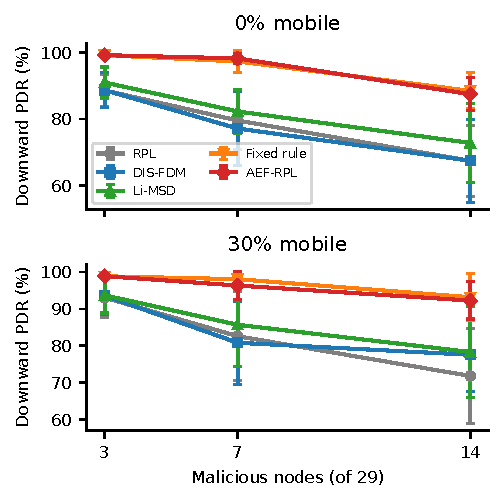
\includegraphics[width=\columnwidth]{full_paper/generated/main_service.pdf}
\caption{Downward delivery under the combined attack by attacker count and mobility (means and 95\% intervals, ten seeds).}\label{fig:service}
\end{figure}

\begin{figure*}[t]
\centering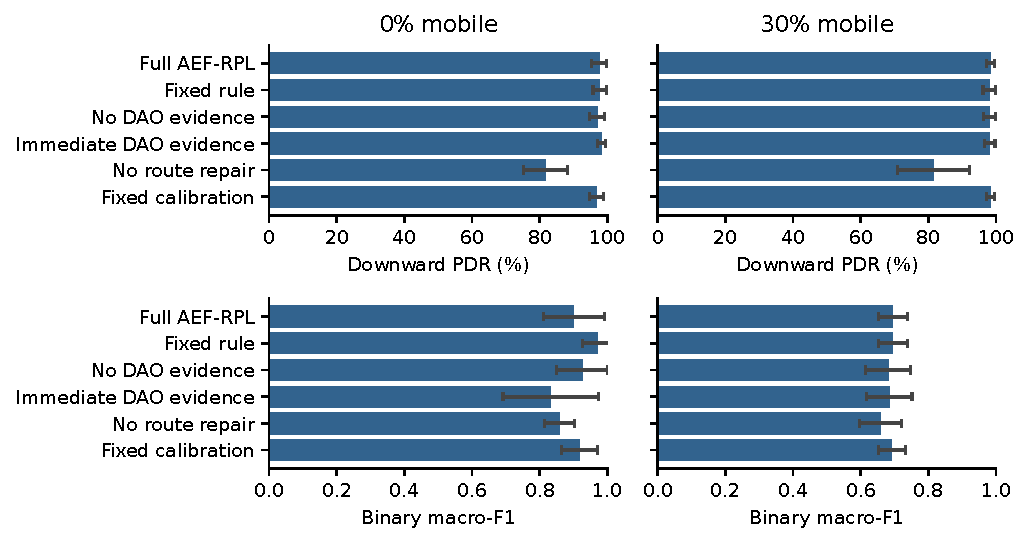
\includegraphics[width=.9\textwidth]{output/experiments/journal_extension/figures/component_ablation.pdf}
\caption{Component ablations under the combined attack (seeds 31--40): macro-F1 with 95\% intervals. ``No dao evidence'' disables only the fused DAO mass; ``no route repair'' keeps detection and blacklisting but drops the repair step.}\label{fig:ablation}
\end{figure*}

\subsection{H4: On-Node Learning}
Learning made decisions faster. With the same evidence, the Q-learning layer lowered the mean latency to the first flag in all six combined-attack conditions ($p_H=.012$): by 20--27\% in static networks (26.4~s against 33.0~s with seven attackers) and by 53--73\% in mobile networks (14.0~s against 32.9~s; Table~\ref{tab:primary}). ARI did not decrease significantly in any condition, so the faster decisions cost no service.

Learning did not lower false positives. FPR was not significantly lower in any of the eight tested conditions, and on the twenty fresh benign mobile runs it was 42.41\% with learning against 42.07\% without (paired difference 0.34 points, interval 0.00--1.03, $p=1.0$). In nine of the ten fresh seeds, both versions flagged the same number of honest nodes. The false isolations therefore do not come from the decision layer, which only chooses between the actions the evidence suggests. They come from the parent-change evidence inherited from DIS-FDM: a mobile node that changes parents legitimately looks like an attacker, and the learner's reward, built from the same local indicators, confirms that choice instead of correcting it. The action logs show the cost of this feedback loop. Learning performed 1352.7 blacklist operations per benign run against 204.1 for the fixed rule, repeatedly releasing and re-isolating the same neighbors. In the ablation, learning off reached a higher static macro-F1 (.971 against .901) with a lower FPR (3.2\% against 11.8\%), and both variants were equal under mobility (.695). H4 is not supported for false positives, while the learning layer did produce a significant latency benefit.

\subsection{H5: Consistency Across Conditions}
The service effect held in every tested condition. In the main campaign, it was significant at every attacker fraction in both static and mobile networks (Table~\ref{tab:primary}). The fresh-seed campaign replicated it on networks not used during design. At the default rate, AEF-RPL reached 95.7\% downward PDR in static and 98.0\% in mobile networks against 78.7\% and 82.8\% for DIS-FDM, paired differences of 17.0 points (bootstrap interval 13.2--21.2) and 15.2 points (7.2--23.7). ARI followed the same pattern (Table~\ref{tab:extension}). Every seed favored AEF-RPL in these cells (exact sign-flip $p=.002$). After Holm adjustment across all tests of the rate study, $p_H=.172$, so the confirmatory inference rests on the pre-specified main-campaign tests, and the fresh seeds replicate the direction and size of the effect.

\begin{table}[t]
\caption{Fresh-seed replication at the default rate (seven attackers, seeds 21--30).}\label{tab:extension}
\centering\footnotesize\begin{tabular}{@{}lrrrr@{}}
\toprule
Mobile (\%) & Method & Macro-F1 & ARI & New recall \\
\midrule
0 & DIS-FDM & 0.939 & 0.741 & 0.986 \\
0 & Li-MSD & 0.974 & 0.791 & 0.943 \\
0 & AEF learning & 0.912 & 0.921 & 0.986 \\
30 & DIS-FDM & 0.641 & 0.800 & 1.000 \\
30 & Li-MSD & 0.925 & 0.847 & 0.800 \\
30 & AEF learning & 0.647 & 0.986 & 1.000 \\
\bottomrule
\end{tabular}

\end{table}

Across attack rates and reception loss (Figs.~\ref{fig:rates} and~\ref{fig:radio}), the paired difference with DIS-FDM was positive with a bootstrap interval above zero in 10 of 12 cells. Reception loss did not erase the gain: at 80\% reception success, the static difference grew to 20.5 points. The two exceptions were the slowest attack (DIS and DAO every 30~s), where every configuration, including no defense, delivered 80--86\% downward. At that rate, AEF-RPL still identified 98.6\% of static and 100\% of mobile attackers, against 2.9\% and 44.3\% for DIS-FDM and at most 1.4\% for Li-MSD, but detection no longer translated into restored service. Mobility consistently raised FPR for every method that uses parent-change evidence (45.0\% for AEF-RPL and 45.9\% for DIS-FDM in the fresh-seed mobile cell), against 0\% for Li-MSD, which does not use it. H5 is supported for the service effect.

\begin{figure*}[t]
\centering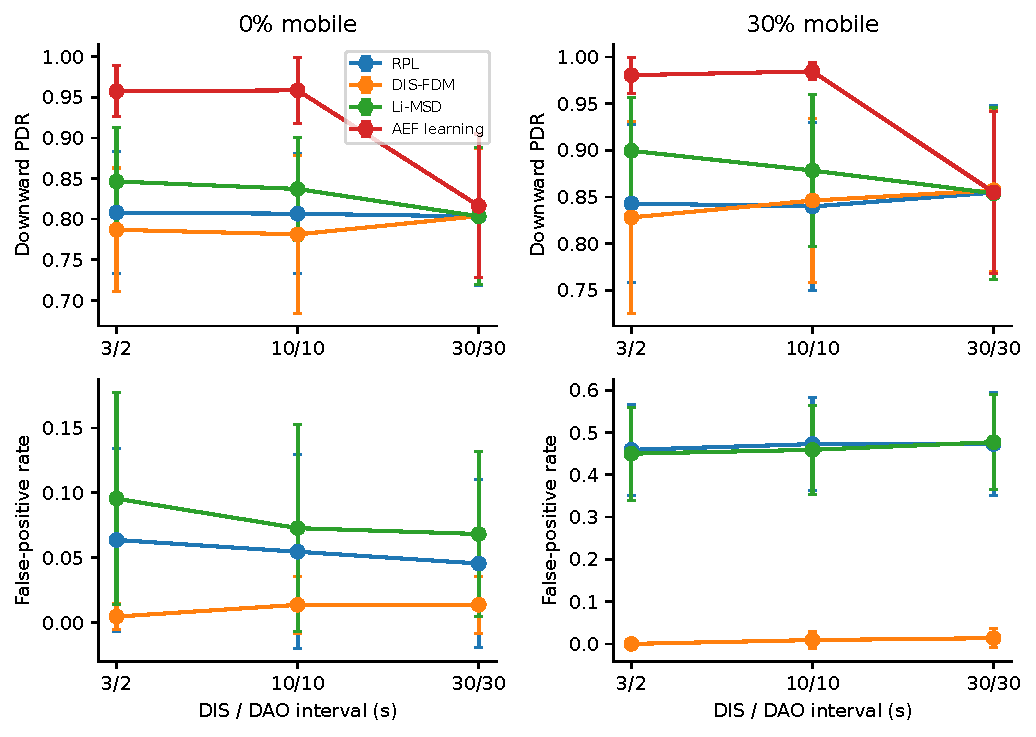
\includegraphics[width=.84\textwidth]{output/experiments/journal_extension/figures/rate_robustness.pdf}
\caption{Attack-rate robustness (seven attackers, seeds 21--30): downward PDR (top) and FPR (bottom). DIS and DAO intervals change together.}\label{fig:rates}
\end{figure*}

\begin{figure}[t]
\centering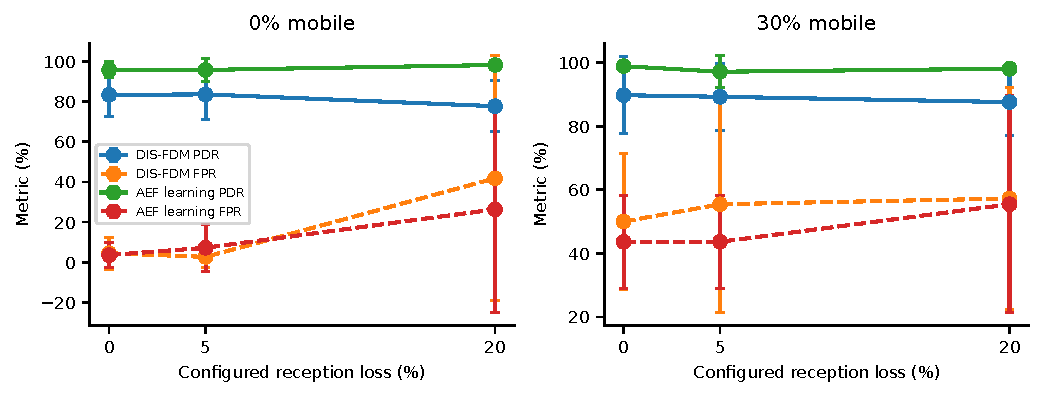
\includegraphics[width=\columnwidth]{full_paper/generated/radio_loss.pdf}
\caption{Reception-loss robustness (seeds 41--45): downward PDR (solid) and FPR (dashed) versus configured reception loss.}\label{fig:radio}
\end{figure}

\subsection{Cost}
AEF-RPL added little computation. On the host, the median per-window callback time averaged 2.57~$\mu$s for AEF-RPL against 2.02~$\mu$s for DIS-FDM in static attacked runs, and 5.15 against 3.51~$\mu$s in mobile runs; the 95th percentiles were 7.06 against 5.26~$\mu$s and 10.28 against 7.06~$\mu$s. AEF-RPL also lowered the estimated transmit power of the attacked network (0.126~mW against 0.182~mW for DIS-FDM with three static attackers). The learning state adds 780~bytes per node.

\begin{table*}[t]
\caption{Hypothesis decisions. Evidence counts the conditions in which the effect was significant ($p_H<.05$) out of those tested, unless noted.}\label{tab:hypotheses}
\centering\footnotesize\begin{tabularx}{\textwidth}{@{}l>{\raggedright}p{0.24\textwidth}X>{\raggedright\arraybackslash}p{0.17\textwidth}@{}}
\toprule
Hyp. & Alternative hypothesis ($H_1$) & Evidence (significant conditions / tested, Holm $p<.05$) & Decision\\
\midrule
H1 & DIS-FDM's published trends are reproduced & 4/8 effect directions & Partly supported \\
H2 & Combined attack is worse than each single attack & Down PDR vs DIS 6/6; DIO vs DAO 5/6; ARI vs DIS 6/6, vs DAO 0/6 & Partly supported \\
H3 & AEF-RPL outperforms DIS-FDM against the combined attack & Down PDR 6/6; ARI 6/6; TPR 0/6; FPR higher 0/6; DAO-only TPR 4/6 & Supported for service; detection at parity \\
H4 & Learning lowers FPR without lowering ARI & FPR lower 0/8; ARI lower 0/6; latency lower 6/6 & Not supported (FPR); latency gain \\
H5 & Effects hold across seeds, topologies, rates and radio loss & Static 3/3, mobile 3/3; extension cells with CI $>0$ 10/12 & Supported for service \\
\bottomrule
\end{tabularx}

\end{table*}

\subsection{Summary of Key Findings}
\begin{itemize}
\item DIS-FDM's control-overhead mechanism was reproduced; its delivery losses were not, because of the always-on MAC (H1).
\item The combined attack added DIS overhead and DAO route loss without amplifying either (H2).
\item AEF-RPL raised downward PDR and ARI over DIS-FDM in all six conditions, with equal detection and no significant FPR increase. Selective DAO repair produced most of the gain (H3).
\item On-node learning cut detection latency by 20--73\% in every condition but did not reduce false isolation, which originates in the parent-change evidence (H4).
\item The service gain held across seeds, attacker fractions, mobility, attack intervals up to 10~s, and reception loss (H5).
\end{itemize}
